\section{Swagger}
%Spiegazione come è stata creata la grafica per gli endpoint con screen di un'interfaccia Controller.

Swagger è un framework utilizzato per la documentazione, progettazione e gestione di API REST.
Per garantire ordine sul mio lavoro e una comunicazione più trasparente e chiara con chi lavora nel lato Front-End è stato creato questo documento utilizzando lo standard OpenAPI.\\
Questo disegno dell'API ha sostituito poi il mock iniziale dell'API, considerando questo nuovo documento come unico per la consultazione dell'API finale.
\begin{figure}[H] 
    \centering 
    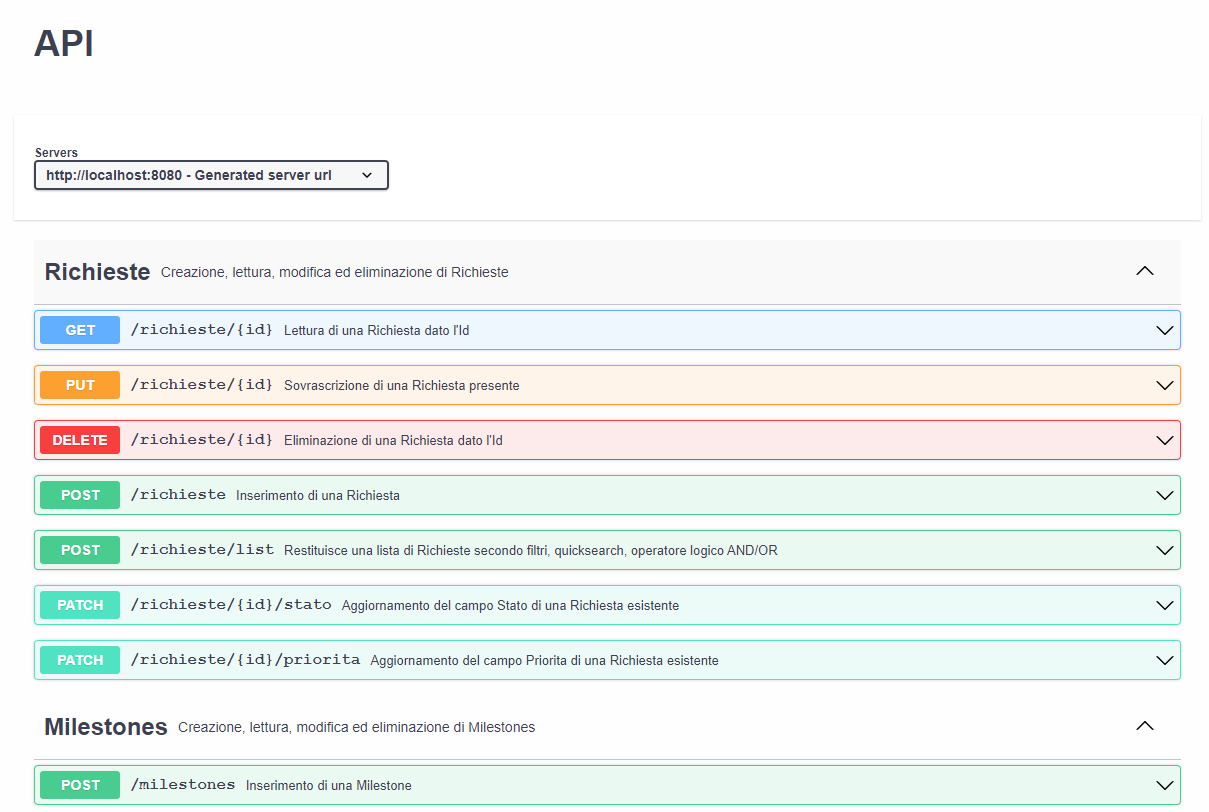
\includegraphics[width=0.95\columnwidth]{foto-swagger-titolo} 
    \caption{Inizio del documento di definizione dell'API}
\end{figure}
\noindent Il documento rappresenta un disegno completo dell'implementazione dell'API REST. Contiene tutti gli endpoint sviluppati, come sono strutturati al loro interno e arrichito di descrizioni per endpoint, risposte, richieste ed errori.
\begin{figure}[H] 
    \centering 
    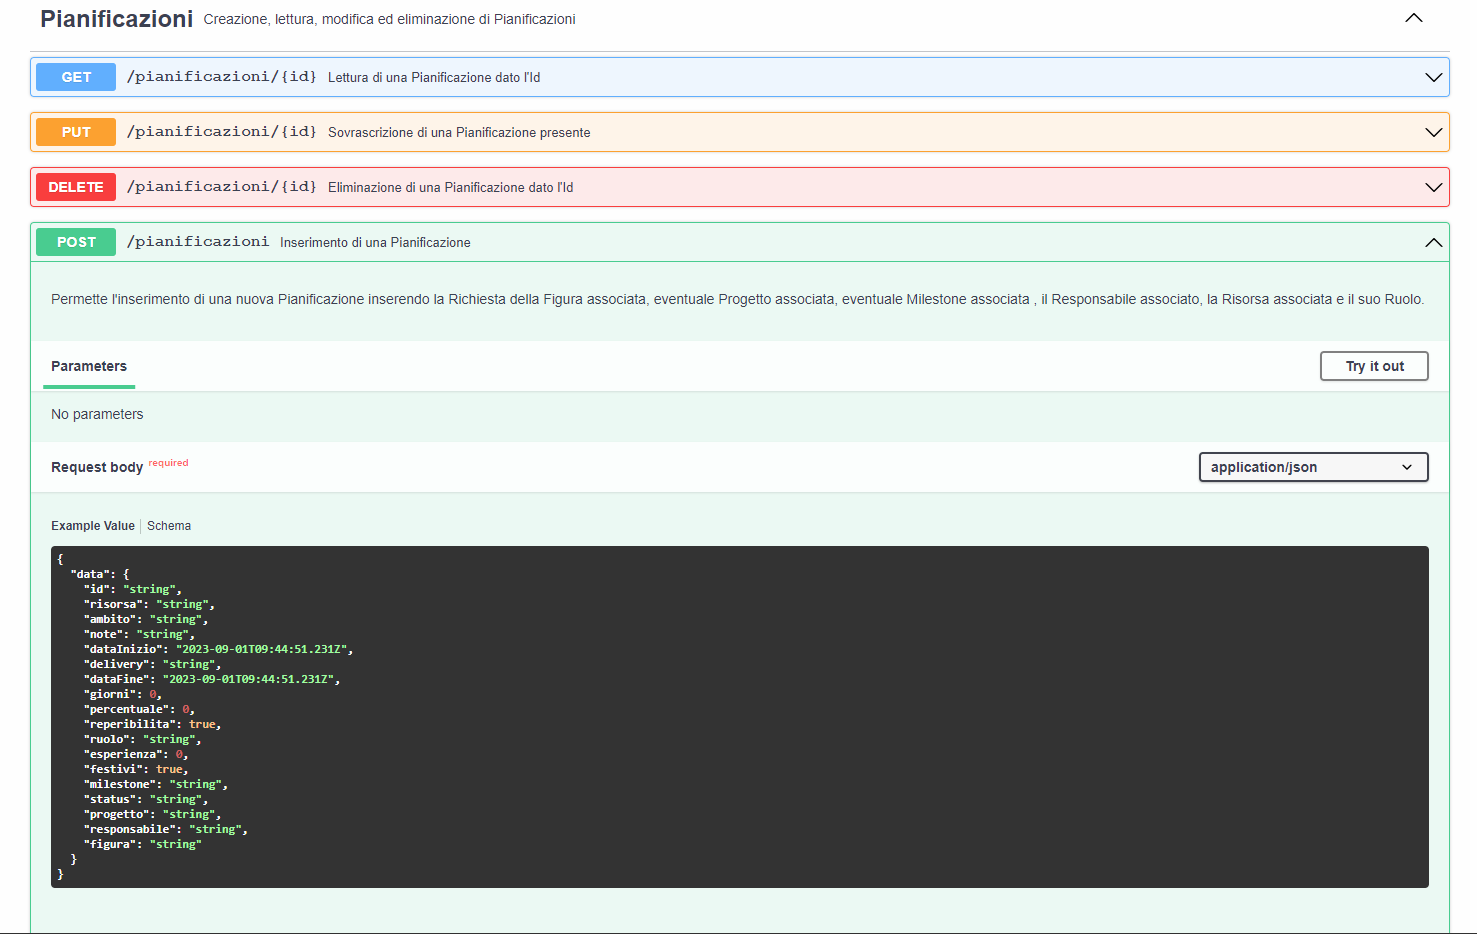
\includegraphics[width=0.95\columnwidth]{foto-swagger-example-value-2} 
    \caption{Example value del body richiesto dall'endpoint}
\end{figure}
\noindent In questa immagine possiamo notare un "Example value" del body richiesto da parte dell'endpoint POST /pianificazioni.\\
\begin{figure}[H] 
    \centering 
    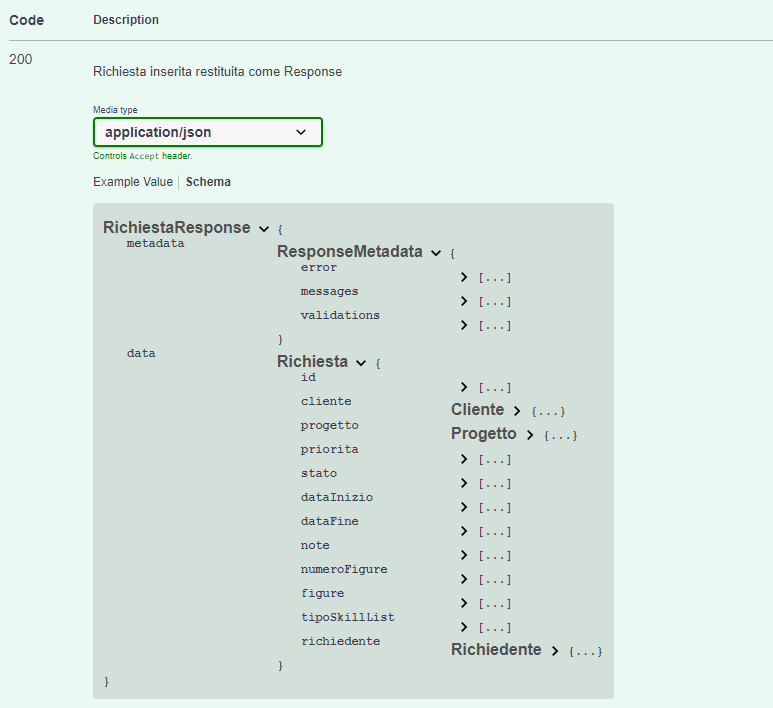
\includegraphics[width=0.65\columnwidth]{foto-swagger-composizione-oggetto} 
    \caption{Composizione oggetto response ritornato dall'endpoint}
\end{figure}
\noindent Inoltre, è possibile esaminare la struttura di ciascun oggetto, sia nelle richieste che nelle risposte. Questo è particolarmente vantaggioso per gli sviluppatori Front-End, poiché consente loro di interagire in modo accurato con il Back-End. In questo modo, il Back-End indica al Front-End cosa e come ci si aspetta di ricevere per quanto riguarda i dati nelle richieste, mentre il Front-End viene informato su come e cosa riceverà dal Back-End nelle risposte.
\begin{figure}[H] 
    \centering 
    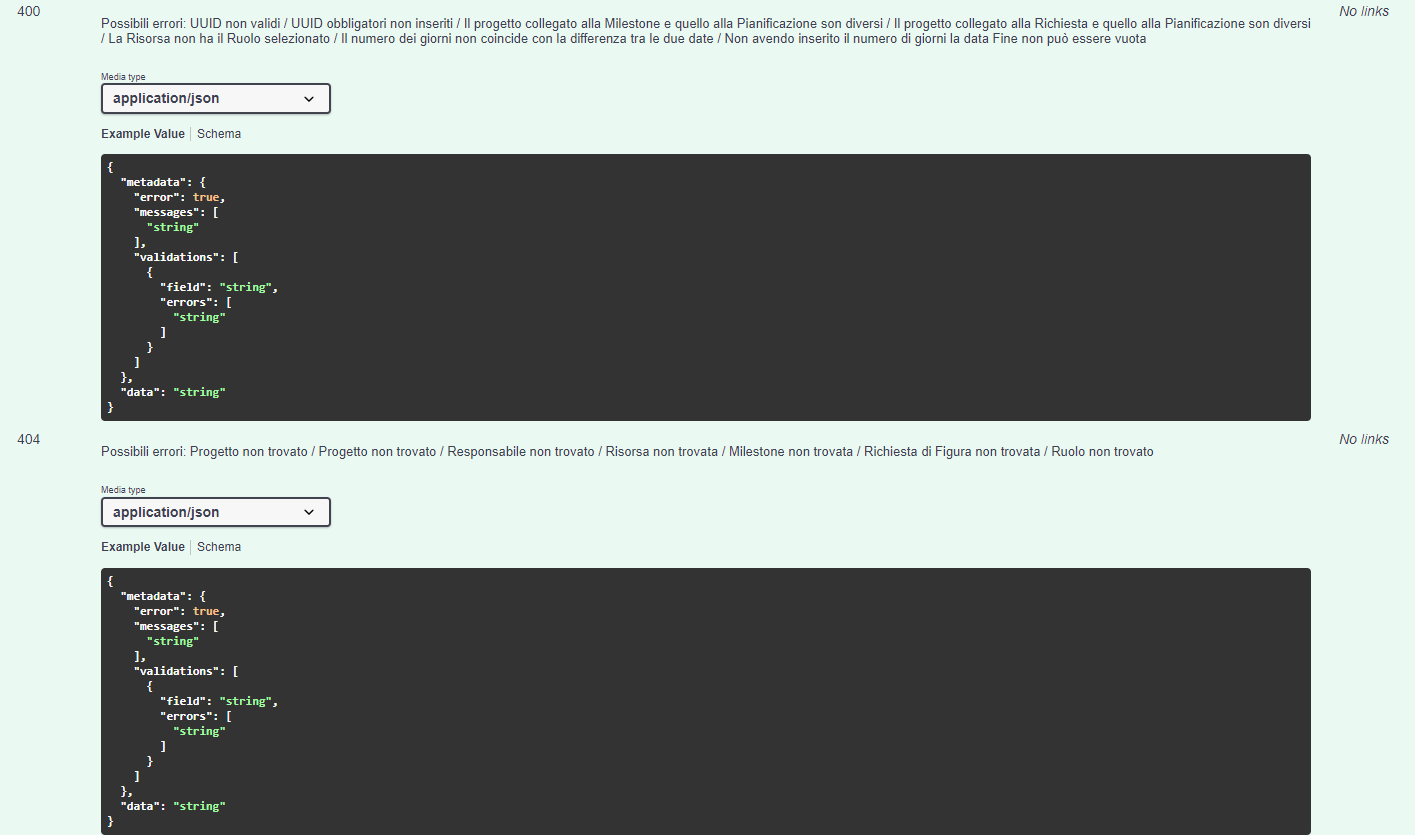
\includegraphics[width=1.00\columnwidth]{foto-swagger-errori} 
    \caption{Errori possibili in un endpoint}
\end{figure}
\noindent Per garantire una comprensione chiara dei possibili errori che potrebbero verificarsi, vengono identificate e descritte varie situazioni, ciascuna associata a un codice di errore specifico, al fine di fornire una struttura generale per codice di errore.

\subsection{Generazione automatica del documento}
Per creare la documentazione dell'API è stata utilizzata la dipendenza \textit{springdoc-openapi-starter-webmvc-ui} citata nella sotto-sezione \hyperlink{doc-api}{4.7.2.1} nel capitolo di Progettazione. Grazie a questa dipendenza è stato possibile generare automaticamente la documentazione dell'API basata sulle annotazioni presenti nel codice sorgente. SpringDoc API utilizza le annotazioni di Spring per identificare i Controller, i metodi delle API, i dati in input e in output. Per visualizzare questo documento generato è possibile accederci tramite un endpoint specifico: \textit{https://localhost:porta\_scelta/swagger-ui.html}.
\begin{figure}[H] 
    \centering 
    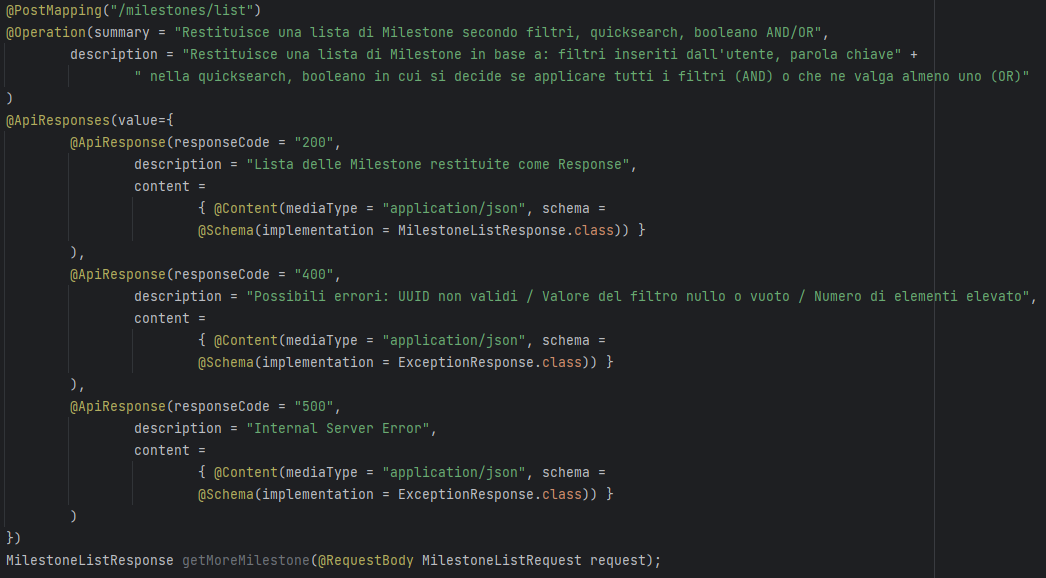
\includegraphics[width=0.90\columnwidth]{api-doc-annotazioni} 
    \caption{Annotazioni utili a generare la documentazione per l'API}
\end{figure}
\noindent La dipendenza importata fornisce anche annotazioni per arrichire il documento. In questa immagine notiamo le seguenti annotazioni:
\begin{itemize}
\item \textit{@Operation}, specifica un sommario dell'endpoint che l'utente può vedere prima di visualizzare nella sua totalità l'endpoint e un campo descrizione per fornire una descrizione più approfondita sul funzionamento;
\item \textit{@ApiResponses}, formata da tanti \textit{@ApiResponse} che specificano il codice di errore, la descrizione di quando questo errore esce e lo schema che avrà quando si presenterà.
\end{itemize}
Per agevolare la lettura dell'API è stata anche utilizzata la notazione \textit{@Schema} per fornire un nome appropriato a campi o classi.






